\section{Simulieren}

\subsection{Die Entstehung von Galaxien}
\par ''Eine Galaxie ist eine durch Gravitation gebundene große Ansammlung von
Sternen, Planetensystemen, Gasnebeln und sonstigen Stellaren Objekten.''
\footnote{\url{https://de.wikipedia.org/wiki/Galaxie}}

\par Demnach ist es relativ Einfach eine Galaxie zu generieren: es werden
einfach ganz viele Objekte in einen Raum geworfen. Das reicht jedoch nicht um
die Objekte als Galaxie definieren zu können, da sie nicht ''durch Gravitation
gebunden'' sind.

\par Um dies zu tun muss die Kraft zwischen allen Objekten in der Galaxie
berechnet werden um damit die Position der jeweiligen Objekte nach einer
bestimmten Zeit bestimmen zu können.

\par Tut man dies, indem man zwischen allen Objekten die Kräfte berechnet kommt
es zu Problemen: die Anzahl der Kraft Berechnungen die durchgeführt werden
müssen steigen exponentiell: Die Anzahl der Kräfte die auf \(n\) Sterne wirken
lassen sich mit der Formel \( n \cdot (n-1) \) berechnen. Für \( n=3 \) müssen
demnach \( 6 \) Kräfte berechnet werden, für \( 100 \) Sterne dagegen \( 9900
\) und für \( 1.000.000 \) Sterne \( \approx 9.99999 \cdot 10^{11} \). Die
Anzahl der Kraft Berechnungen, die durchgeführt werden müssen beim Simulieren
einer ''echten'' Galaxie mit \( > 200 \cdot 10^6 \) Sternen ist demnach so
groß, dass die Anzahl der Kräfte die berechnet werden müssen minimiert werden
müssen, um in einer sinnvollen Zeit an ein Ergebnis zu kommen.

\par Dies reicht jedoch auch nicht, um eine ''stabile'' Galaxie zu generieren:
berechnet man nur die Kräfte die auf ruhende Objekte in einem Reibungsfreiem
Raum wirken, würden alle Objekte zum Massen Mittelpunkt gezogen werden und die
Galaxie würde somit implodieren. Es ist also nötig auf die Sterne in der
Galaxie Anfangs Kräfte zu wirken. Diese Kräfte sind durch die Rotation der
Galaxie um den Massen Mittelpunkt der Galaxie definiert, man rotiert also die
Galaxie und gleicht durch die Zentripetalkraft die Kraft die alle Sterne
Richtung Massen Mittelpunkt zieht aus. Rotiert man die Galaxie jedoch zu
schnell, explodiert sie förmlich, da die Sterne nicht mehr zusammengehalten
werden und die Fliehkraft sie einfach auseinanderzieht.

\subsection{Konzepte}

\subsubsection{Zu lösende Probleme}
Wie bereits in der Einleitung beschrieben, ist eines der Probleme das Auftritt
die Anzahl der nötigen Kraft Berechnungen wodurch der Rechenaufwand quadratisch
in Relation zu der Anzahl der Sterne steigt und somit in \( O(n \cdot (n - 1))
\in O(n^2) \) liegt.

\par Es kommt ebenfalls zu Problemen, wenn der mittlere Fehler, der bei der
Berechnung der Kraft entsteht, größer als die wirkende Kraft wird. Dies
passiert unter anderem dann, wenn der Abstand zwischen den Sternen so groß
wird, dass die wirkende Kraft so gering ist das sie mithilfe von Computern
nicht mehr sinnvoll dargestellt werden kann. Statt nun mit Rundungsfehlern zu
rechnen, können diese Sterne, die sehr weit entfernt vom Stern dessen Kräfte
berechnet werden sollen, einfach nicht mehr beachtet werden, da sie nicht
sinnvoll beitragen. Um diese Sterne jedoch nicht komplett aus der Berechnung
auszunehmen, können kleine Cluster an Sternen, welche weit genug vom Stern auf
den die Kräfte berechnet werden sollen weg sind und klein genug sind zu einem
Pseudo-Stern zusammengefasst werden, welcher durch den Masse Mittelpunkt der
Sterne die er repräsentiert definiert ist. Das Konzept wurde 1986 von Josch
Barnes und Piet Hut veröffentlicht \cite{barneshut86} und erlaubt es die Anzahl
an Kräften, die berechnet werden müssen von \( O(n^2) \) auf \( O(n log(n)) \)
zu reduzieren.

\subsubsection{Generierung von Quadtrees und entsprechende Bäume}
Um Sterne clustern zu können muss die Galaxie in der sich die Sterne befinden
in Zellen unterteilt werden. Dazu wird ein Quadtree bzw. Octree (ein k-närer
Baum mit 4 bzw. 8 Kindern) aufgebaut, indem die Sterne eingefügt werden. Damit
die Stern-cluster gebildet werden können müssen die Sterne sich in den Blättern
des Baumes befinden. Die Knoten des Baumes, indem sich die Sterne befinden
dürfen somit keine weiteren Kinder besitzen.

\par Ein Galaxie wie in Abbildung \ref{fig:cells} dargestellt wird demnach
Stern für Stern in einen anfangs leeren Baum eingefügt. Die Größe der ersten
Zelle die nach dem einfügen aller Sterne alle Sterne beinhaltet kann falls
bekannt ist in was für einem Intervall die Koordinaten der Sterne sich befinden
direkt genutzt werden, um die Größe der Zelle zu definieren, andernfalls muss
diese erst ermittelt werden, indem die minimal und maximal Koordinaten in der
liste an Sternen gesucht werden. Beim Einfügen kann es jedoch wie in Abbildung
\ref{fig:insertwithexisting} zu sehen zu Problemen kommen. Im falle, dass der
Knoten, indem ein Stern eingefügt werden soll bereits durch einen anderen Stern
belegt ist müssen für den jeweiligen Knoten Kinder-Knoten erzeugt werden in den
die beiden Sterne eingefügt werden müssen. Dies wird so lange fortgeführt bis
sich alle Knoten in den Blättern des Baums befinden.

\par Eine Zelle ist durch ihren Mittelpunkt und ihrer Breite definiert, daher
verschiebt sich eine Zelle, welche sich eine Ebene ''tiefer'' befinden um ein
Viertel ihre Breite und die Breite der neuen Zelle ist im Relation zu der
ursprünglichen Zelle gesehen halbiert.

\par Nachdem alle Sterne in einen Baum eingefügt wurden und sich in den
Blättern des Baumes befinden, wird der Baum rekursiv durchlaufen und es wird
für jeden inneren Knoten (Knoten, welche keine Blätter sind) die gesamt Masse
ihrer Kinder berechnet und der Massen Mittelpunkt.

\subsubsection{Funktion des Barnes-Hut Algorithmus}
Um nun zu definierten, welche Cluster zusammengefasst werden und welche nicht
wird der Barnes-Hut Algorithmus (\ref{eq:barnes_hut}) verwendet. Dieser
berechnet einen Wert \( \theta \) welcher als Referenz dafür genommen werden
kann, wie die Relation zwischen der Entfernung zu einem Cluster und der Größe
des Clusters ist. Um nun Cluster welche weit genug von einem Stern weg sind und
gleichzeitig klein genug sind zu erkennen und herauszufiltern kann der
Algorithmus in Kombination mit einem vordefinierten Grenzwert genutzt werden.

\begin{figure}[!h]
\centering
\subfloat[Ein Cluster auf mehreren Sternen]{
    \centering
    \begin{tikzpicture}
        \tikzstyle{circlestyle}=[shape=circle,thick,fill,draw, inner sep=0cm]
        \node at (0, 0) {};
        \node at (9, 0) {};

        % Random seed for RNG
        \pgfmathsetseed{7};

        \foreach \x in {1,...,40}
        {
          % Find random numbers
          \pgfmathrandominteger{\a}{10}{390}
          \pgfmathrandominteger{\b}{10}{390}

          % Scale numbers nicely
          \pgfmathparse{0.005*\a}\let\a\pgfmathresult;
          \pgfmathparse{0.005*\b}\let\b\pgfmathresult;

          % draw the circle
          \fill (\a, \b) circle (0.03);
        };

        % draw a box around the star cluster
        \draw[] (0,0) rectangle (2, 2);
        \node[] at (1, 1) (A1) {};
        \draw[arrows=<->] (0,-0.2) -- node[midway, align=center, below] {\(d\)} (2,-0.2);

        % draw a star in the far right of the image
        \node[circlestyle, minimum size=2pt, label=above:\(s_1\)] at (8, 1) (A2) {};

        % draw a line in between the box and the far right of the image
        \draw[dashed, arrows=<->] (A1) -- node[midway, align=center, above] {\(r\)} (A2);
    \end{tikzpicture}
    \label{subfig:ungrouped}
}
\hfill
\subfloat[Die abstraction des obigen Clusters]{
    \centering
    \begin{tikzpicture}
        \tikzstyle{circlestyle}=[shape=circle,thick,fill,draw, inner sep=0cm]
        \node at (0, 0) {};
        \node at (9, 0) {};

        % draw a big star in the far left of the image
        \node[circlestyle, minimum size=2pt, label=above:\(q_1\)] at (1, 0) (B1) {};

        % draw the right star
        \node[circlestyle, minimum size=2pt, label=above:\(s_1\)] at (8, 0) (B2) {};
        
        % draw a line in between the far left star and the right star
        \draw[dashed, arrows=<->] (B1) -- node[midway, align=center, above] {\(r\)} (B2);
    \end{tikzpicture}
    \label{subfig:grouped}
}
\caption{Visuelle Darstellung der Funktionsweise des Barnes-Hut Algorithmus.
Das Stern Cluster aus \ref{subfig:ungrouped} wird in \ref{subfig:grouped} zu einem
Stern abstrahiert.}
\end{figure}

\begin{equation}
\label{eq:barnes_hut} \theta = \frac{d}{r}
\end{equation}

Ist das Verhältnis zwischen Entfernung \( r \) und Breite \( b \) des Clusters
kleiner als der vorher definierte Grenzwert, kann das Cluster zu einem
Pseudostern zusammengefasst werden.

\subsection{Kraft-Berechnungen}

\subsubsection{Die Kraft als Vektor}
Um die Kraft als Vektor zu berechnen, welcher ein Stern B auf einen Stern A
ausübt, wird die folgende Formel verwendet:

\begin{equation}
    \vec{F}_{AB} = \underbrace{-G \frac{m_A m_B}{|r_{AB}|^2}}_{Scalar}
    \cdot \underbrace{\frac{r_B - r_A}{|r_B - r_A|}}_{Vector}
\end{equation}

Die Summe der Kräfte, die auf einen Stern wirken ist somit die Summe aller
Kräfte die zwischen dem jeweiligen Stern \( a \) und allen anderen Sternen
wirken:

\begin{equation}
    F_{a} = \sum_{\substack{i=0 \\ i\neq a}}^{n-1} F_{ai}
\end{equation}

\subsubsection{Berechnung der auf einen Stern wirkenden Kraft}
\par Um die Kraft, welche auf einen bestimmten Stern wirkt, zu berechnen, wird der
Baum von der Wurzel aus rekursiv durchlaufen. Es wird für jeden Knoten das
jeweilige \( \theta \) berechnet und mit dem vorher definierten Grenzwert
verglichen. Ist das berechnete \( \theta \) kleiner als der vorher definierte
Grenzwert wird die Rekursion nicht weiter in den Baum gehen, sondern den
jeweiligen Teilbaum zusammenfassen.

\par Es ist somit durch den Grenzwert somit eine End-Bedingung gegeben, welche
verhindert das zu weit in den Baum vorgedrungen wird und somit auch verhindert,
dass Sterne die in einer zu großen Entfernung zu des Ursprungs Stern liegen und
dicht genug gruppiert sind in die Berechnung miteinbezogen werden.

\par Möchte man die Kraft auf den Stern \( F \) in Abbildung \ref{fig:cells}
berechnen berechnet man das \( \theta \) zwischen \( F \) und dem Wurzel-Knoten. Ist
das berechnete \( \theta \) größer als der vorher definierte Grenzwert kann statt
weiter in den Baum hineinzugehen und weitere Kräfte zu berechnen die Kraft
zwischen \( F \) und dem Pseudostern, der durch den Wurzel-knoten dargestellt wird
direkt berechnet werden. Andernfalls wird weiter in den Baum hineingegangen und
auf der nächsten Baum-Ebene das Entsprechende \( \theta \) zwischen den Sternen
berechnet werden.

\par Betrachtet man Abbildung \ref{fig:cells} fällt auf das die Zelle in der
sich die Sterne \( C \) und \( D \) befinden sehr klein ist und die Entfernung
zu dem Stern \( F \) vergleichsweise hoch ist. Es kann also angenommen werden,
dass das Theta zwischen \( F \) und der Zelle in der sich \( C \) und \( B \)
befinden sehr klein ist. Die Sterne können demnach zusammengefasst werden.

\bigskip

\begin{figure} 
\hspace{1.5cm}
\begin{minipage}{0.45\textwidth}
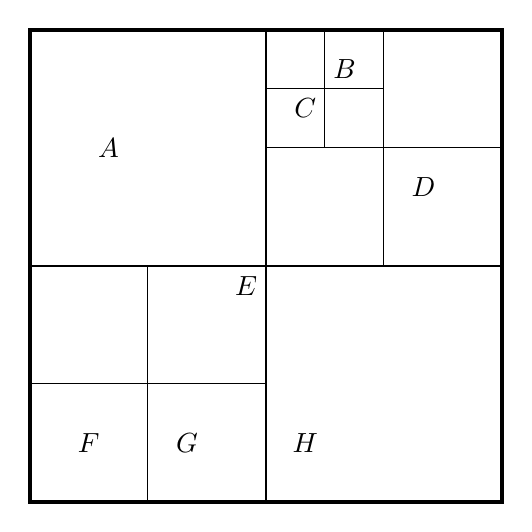
\begin{tikzpicture}[level 1/.style={level distance=1.5cm}]
    % First Layer
    \draw [line width=0.5mm] (0, 0) rectangle (6, 6);

    % Second Layer 
    \draw [line width=0.25mm] (0, 0) rectangle (3, 3);
    \draw [line width=0.25mm] (3, 0) rectangle (6, 3);
    \draw [line width=0.25mm] (0, 3) rectangle (3, 6);
    \draw [line width=0.25mm] (3, 3) rectangle (6, 6);

    % Third Layer (South West)
    \draw [line width=0.125mm] (0, 0) rectangle (1.5, 1.5);
    \draw [line width=0.125mm] (1.5, 1.5) rectangle (3, 3);

    % Third Layer (North East)
    \draw [line width=0.125mm] (3, 3) rectangle (4.5, 4.5);
    \draw [line width=0.125mm] (4.5, 4.5) rectangle (6, 6);

    % Forth Layer (North West)
    \draw [line width=0.125mm] (3, 4.5) rectangle (3.75, 5.25);
    \draw [line width=0.125mm] (3.75, 5.25) rectangle (4.5, 6);

    % Draw the nodes
    \node at (1, 4.5) {$A$};
    \node at (4, 5.5) {$B$};
    \node at (3.5, 5) {$C$};
    \node at (5, 4) {$D$};
    \node at (2.75, 2.75) {$E$};
    \node at (0.75, 0.75) {$F$};
    \node at (2, 0.75) {$G$};
    \node at (3.5, 0.75) {$H$};
\end{tikzpicture}
\end{minipage}
\caption{Unterteilung einer Galaxie in verschiedene Zellen}
\label{fig:cells}
\end{figure}

\begin{figure}
\centering
\begin{forest}
    for tree={circle,draw, s sep+=0.25em}
    [
        [A]
        [
            [
                []
                [B]
                [C]
                []
            ]
            []
            []
            [D]
        ]
        [
            []
            [E]
            [F]
            [G]
        ]
        [H]
    ]
\end{forest}
\caption{Die in Abbildung \ref{fig:cells} dargestellte Galaxie als Baum
dargestellt}
\end{figure}


\begin{figure}
\subfloat[Anfangszustand. Der Stern B soll in den Baum, indem sich bereits A befindet, eingefügt werden.]{
    \begin{forest}
        for tree={circle,draw, s sep+=0.25em}
        [,phantom
            [B]
            [
                A
            ]
        ]
    \end{forest}
}
\,
\subfloat[Stern B kann nicht eingefügt werden, da der Slot durch A belegt ist, also wird A weiter in den Baum versickert.]{
    \begin{forest}
        for tree={circle,draw, s sep+=0.25em}
        [,phantom
            [B]
            [
                [A]
                []
                []
                []
            ]
        ]
    \end{forest}
}
\,
\subfloat[B wird nun eingefügt, da sich B jedoch nicht in einem Blatt befinden, muss B weiter versickert werden.]{
    \begin{forest}
        for tree={circle,draw, s sep+=0.25em}
        [,phantom
            [B
                [A]
                []
                []
                []
            ]
        ]
    \end{forest}\quad\\[2ex]
}
\,
\subfloat[Damit B versickert werden kann, wird der Platz der durch A besetzt wird freigemacht, indem A weiter versickert wird.]{
    \begin{forest}
        for tree={circle,draw, s sep+=0.25em}
         [B
             [
                 [A]
                 []
                 []
                 []
             ]
             []
             []
             []
         ]
    \end{forest}\quad
}
\,
\subfloat[B kann jetzt in den Baum versickert werden und ist nun ein Blatt.]{
    \begin{forest}
        for tree={circle,draw, s sep+=0.25em}
         [
             [
                 [A]
                 []
                 [B]
                 []
             ]
             []
             []
             []
         ]
    \end{forest}\quad
}

\caption{Schrittweises einfügen des Sternes B in einen Baum, indem sich bereits ein Stern (A) befindet.}
\label{fig:insertwithexisting}
\end{figure}

\subsection{Stabile Galaxien}
Um eine stabile Galaxie zu generieren muss diese rotiert werden damit die
Zenrtifugalkraft der Kraft welche die Sterne zum Massemittelpunkt zieht
entgegenwirkt. Dies lässt sich einfach berechnen, jedoch entsteht ein großes
Problem: Es muss eine Kraft ermittelt werden welche am Anfang der Simulation
wirkt.

\par Da das Ziel meines Projektes nicht darin liegt das Anfangswertproblem zu
untersuchen, sondern die restliche Simulation stark zu verschnellern habe ich
beschlossen das Problem in ein eigenes, einfach austauschbares Modul zu
verpacken und so in der Zukunft einfach austauschbar zu machen.

\par Um jedoch eine ``halb'' Stabile Galaxie zu generieren rotierte ich einfach
(im zwei Dimenionalem) die Kraft die im ersten Zeitschritt auf den Stern wirkte
um 90 Grad. Dadurch rotieren die Sterne anfangs um den Massenmittelpunkt.
Dieses Konzept ist in keinem Sinne physikalisch korrekt, es kann jedoch als
Platzhalter genutzt werden bis einer richtige Möglichkeit gefunden wird dies zu
berechnen.

\subsection{Datenbanken}

\subsubsection{Speichern der Sterne}

Die Sterne werden in einer Tabelle in Datenbank \mbox{PostgreSQL} gespeichert.
Die Tabelle ist wie in Abbildung \ref{fig:stars_table} zu sehen aufgebaut.

\begin{figure}[h!]
\centering
\begin{tabular} {l | l | l | l | l | l}
star\_id & \(x\) & \(y\) & \(vx\) & \(vy\) & \(m\) \\ \hline\hline
1        & -300 & 300 & 0  & 0  & 1000 \\ \hline
2        & -200 & -200 & 0  & 0  & 1000 \\ \hline
\dots   & \dots & \dots & \dots & \dots & \dots \\ \hline
n       & \(x_n\) & \(y_n\) & \(vx_n\)& \(vy_n\) & \(m_n\) \\ \hline
\end{tabular}
\caption{Darstellung der Tabelle in der die Sterne gespeichert werden. Die
star\_id spalte beinhaltet eine global einmalige ID wodurch jeder Stern
identifiziert werden kann.}
\label{fig:stars_table}
\end{figure}

Dadurch das jeder Stern eine einmalige ID besitzt kann diese verwendet werden
um einfach auf Sterne zu verweisen. Dies ist im Kontext des Einfügens sehr
hilfreich da die Verschiebung eines Sternes durch ändern der Stern-ID vollzogen
werden kann.

\par Jeder Stern besitzt eine Position, einer Geschwindingkeit und eine Masse.
Dadurch kann man einen Stern definieren, jedoch auch berechnen was für eine
Kraft der Stern auf andere Sterne auswirkt. 

\subsubsection{Speichern von Bäumen}
Um die Bäume in denen die galaxien giepeichert werden in einer Datenbank zu
speichern, muss eine einheitliche Struktur definiert werden um Probleme in der
Zukunft zu verhindern. Die Nutzung von speziellen Graphen Datenbanken bietet
sich natürlich an, jedoch wird diese starke Spezialisierung schnell zu einem
Hindernis. Um nach dem KISS Prinzip\footnote{"Das KISS-Prinzip (englisch Keep
it simple, stupid) fordert, zu einem Problem eine möglichst einfache Lösung
anzustreben." \url{https://de.wikipedia.org/wiki/KISS-Prinzip}} eine möglichst
einfache Lösung zu nutzen werden die Bäume in einer Relationalen Datenbank
gespeichert. Jeder Knoten wird dabei in einer Zeile der Datenbank gespeichert
und erhält eine global einzigartige ID. Die Kinder in andrem Knoten hängen
werden anhand ihrer ID in der Zeile gespeichert sodass es einfach möglich ist
einfach auf diese zuzugreifen und beim rekursiven durchsuchen des Baumes auf
diese zuzugreifen. Möchte man einen Teilbaum unterteilen können einfach vier
neue Knoten erzuegt werden welche vom Knoten an dem sie hängen referneziert
werden.

\begin{figure*}[ht]
\begin{tabular} {l | l | l | l | l | l | l | l | l | l}
node\_id & box\_width & total\_mass & depth & star\_id & root\_id & isleaf & box\_center & center\_of\_mass & subnodes  \\ 
bigint & numeric & numeric & numeric & bigint & bigint & boolean & numeric[] & numeric[] & numeric[]  \\ \hline\hline
2921847 & 1000 & 2000 & 0 & 0 & 1 & False & \{0, 0\}       & \{0, 0\}       & \{ \(\dots\) \}  \\ \hline
2921848 & 500  & 1000 & 1 & 1 & 1 & True  & \{-500, 500\}  & \{-300, 300\}  & \{ \(\dots\) \}  \\ \hline
2921849 & 500  & 0    & 1 & 0 & 1 & True  & \{500, 500\}   & \{0, 0\}       & \{ \(\dots\) \}  \\ \hline
2921850 & 500  & 1000 & 1 & 2 & 1 & True  & \{-500, -500\} & \{-200, -200\} & \{ \(\dots\) \}  \\ \hline
2921851 & 500  & 0    & 1 & 0 & 1 & True  & \{500, -500\}  & \{0, 0\}       & \{ \(\dots\) \}  \\ \hline
\end{tabular}
\caption{Darstellung der Tabelle in der ein Baum definiert ist, welcher einmal unterteilt wurde.}
\end{figure*}


